% !TEX program = xelatex
% 공통수학2 · Ⅱ. 집합과 명제 · 2. 명제 · 02 명제 사이의 관계 · 2/2차시
\documentclass[11pt,a4paper]{article}
\usepackage{kotex}
\usepackage{iftex}
\ifPDFTeX\else
  \setmainhangulfont{Noto Serif CJK KR}
  \setsanshangulfont{Noto Sans CJK KR}
\fi
\usepackage[margin=2.1cm]{geometry}
\usepackage{parskip}
\usepackage{enumitem}
\usepackage{array}
\usepackage{tabularx}
\usepackage{booktabs}
\usepackage{xcolor}
\usepackage{amssymb}
\usepackage{tikz}
\usepackage[most]{tcolorbox}
\usepackage{fancyhdr}
\usepackage{titlesec}

\definecolor{goldc}{HTML}{B07C22}
\definecolor{goldstrong}{HTML}{8A5F16}
\definecolor{indigoc}{HTML}{2B3B57}
\definecolor{indigosoft}{HTML}{6E82A6}
\definecolor{linec}{HTML}{D6DACB}
\definecolor{surface2}{HTML}{E4E8DC}
\definecolor{notebg}{HTML}{FBF3E3}
\definecolor{inksoft}{HTML}{52604F}

\titleformat{\section}{\normalfont\sffamily\bfseries\large\color{indigoc}}{\thesection}{0.6em}{}
\titlespacing{\section}{0pt}{16pt}{8pt}
\newtcolorbox{ideabox}{enhanced, breakable, colback=white, colframe=goldc, boxrule=0.5pt, leftrule=3pt, arc=2pt, left=10pt, right=10pt, top=8pt, bottom=8pt}
\newtcolorbox{calloutbox}{enhanced, breakable, colback=white, colframe=indigosoft, boxrule=0.5pt, leftrule=3pt, arc=2pt, left=10pt, right=10pt, top=7pt, bottom=7pt}
\newtcolorbox{notebox}{enhanced, breakable, colback=notebg, colframe=goldc, boxrule=0.5pt, leftrule=3pt, arc=2pt, left=10pt, right=10pt, top=7pt, bottom=7pt}
\newtcolorbox{answerbox}{enhanced, breakable, colback=white, colframe=linec, boxrule=0.5pt, arc=2pt, left=10pt, right=10pt, top=7pt, bottom=7pt}
\newcommand{\lessonbanner}[3]{%
  \begin{tcolorbox}[enhanced, colback=indigoc, colframe=indigoc, boxrule=0pt, arc=0pt,
    left=14pt, right=14pt, top=14pt, bottom=10pt, borderline south={2.4pt}{0pt}{goldc}, fontupper=\color{white}]
    {\sffamily\footnotesize\color{white!85!black} #1}\\[4pt]{\sffamily\bfseries\Large #2}\\[3pt]{\sffamily\small\color{white!88!black} #3}
  \end{tcolorbox}}
\pagestyle{fancy}\fancyhf{}\renewcommand{\headrulewidth}{0pt}
\fancyfoot[L]{\footnotesize\color{inksoft} 공통수학2 · 2026학년도 2학기 · 지평선고등학교}
\fancyfoot[R]{\footnotesize\color{inksoft} 교사용 지도안 -- 배포 금지}

\begin{document}
\lessonbanner{공통수학2 · Ⅱ. 집합과 명제 · 2. 명제}{02 명제 사이의 관계 --- 2/2차시}{충분조건과 필요조건 · 교사용 지도안 (2026학년도 2학기)}
\vspace{10pt}

\noindent\begin{tabularx}{\linewidth}{@{}>{\bfseries\color{indigoc}}p{2.6cm}X@{}}
\toprule
대상 & 고1 · 2개 반 · 반당 13명 \\
차시 & 50분 (도입 10 · 전개 30 · 정리 10) \\
성취기준 & 충분조건, 필요조건, 필요충분조건의 뜻을 알고 판별할 수 있다. \\
선행 학습 & 28차시 --- 명제의 역과 대우 \\
\bottomrule
\end{tabularx}

\section{학습 목표 \& Big Idea}
\begin{ideabox}
\textbf{\color{goldstrong}영속적 이해 (Big Idea)}\\
명제 $p\to q$가 참일 때, $p$는 $q$이기 위한 충분조건이고 $q$는 $p$이기 위한 필요조건이다. 두 진리집합이 같으면($P=Q$) 두 조건은 완전히 같은 것을 가리키는 필요충분조건(동치)이 된다.
\vspace{4pt}
\small\color{inksoft} 핵심개념: \textbf{충분·필요} \quad\textbullet\quad 핵심개념: \textbf{동치} \quad\textbullet\quad 일반화: \textbf{조건 사이의 포함 관계가 충분·필요를 결정한다}
\end{ideabox}
\begin{calloutbox}
\textbf{차시 학습 목표}
\begin{itemize}[leftmargin=1.4em, itemsep=2pt, topsep=4pt]
  \item 두 조건의 진리집합 사이의 포함 관계를 이용하여 충분조건, 필요조건, 필요충분조건을 판별할 수 있다.
  \item 세 조건의 진리집합 사이의 포함 관계로부터 참인 명제를 찾을 수 있다.
\end{itemize}
\end{calloutbox}

\section{질문의 연결}
\begin{tabularx}{\linewidth}{@{}>{\bfseries\color{indigoc}\small}p{2.4cm}X@{}}
사실적 질문 & 명제 $p\to q$가 참일 때, $p$와 $q$는 각각 어떤 이름의 조건이라고 부를까? \\[6pt]
개념적 질문 & 왜 진리집합이 서로 같을 때만 `필요충분'이라는 말을 쓸까? 포함 관계와 `충분/필요'라는 이름은 어떻게 연결될까? \\[6pt]
논쟁적 질문 & 일상에서 쓰는 `충분', `필요'라는 말과 수학에서의 뜻은 어떻게 다를까? 이 차이는 왜 생겼을까? \\
\end{tabularx}

\section{수업 흐름}
\begin{tabularx}{\linewidth}{@{}>{\centering\arraybackslash}p{1.6cm}X>{\raggedright\arraybackslash\small}p{3.1cm}@{}}
\toprule
\textbf{단계} & \textbf{활동 \& 발문} & \textbf{ATL / VTR} \\
\midrule
\textcolor{goldstrong}{\textbf{도입}}\newline\footnotesize 10분 &
\textbf{마음공부 (2분)} --- 유무념 대조.\newline
\textbf{생각 열기 (8분)} --- ``$a$는 4의 배수이다.'' $\to$ ``$a$는 2의 배수이다.''는 참인 명제. 이때 두 조건은 서로 어떤 관계일지 예측. &
ATL: 사고(관계 추론)\newline VTR: See-Think-Wonder \\
\addlinespace
\textcolor{goldstrong}{\textbf{전개}}\newline\footnotesize 30분 &
\textbf{충분·필요·필요충분조건 (12분)} --- 기호 $p\Rightarrow q$, $p\Leftrightarrow q$ 도입 $\to$ 정의(충분조건/필요조건/필요충분조건) $\to$ 예제 2($P\subsetneq Q$인 경우와 $P=Q$인 경우 비교).\newline
\textbf{판별 연습 (8분)} --- 문제 4로 진리집합을 구해 포함 관계 판별.\newline
\textbf{탐구 활동 --- 벤 다이어그램 (10분)} --- 세 조건 $p$, $q$, $r$에서 `$p$는 $q$이기 위한 필요조건, $r$은 $q$이기 위한 충분조건'이 주어질 때 $R\subset Q\subset P$를 벤 다이어그램으로 나타내고, 참인 명제를 모두 찾기. &
ATT: 촉진자 역할\newline ATL: 협업(모둠 벤 다이어그램) \\
\addlinespace
\textcolor{goldstrong}{\textbf{정리}}\newline\footnotesize 10분 &
\textbf{개념 연결 질문 (5분)} --- ``세 조건이 $R\subset Q\subset P$ 관계일 때, $r$은 $p$이기 위한 무슨 조건일까?''\newline
\textbf{성찰 (5분)} --- 감사 일기 1문장 + `명제 사이의 관계' 소단원 마무리 + 다음 차시 예고(명제의 증명: 대우증명법, 귀류법). &
마음공부 · 감사 일기 \\
\bottomrule
\end{tabularx}

\begin{calloutbox}
\textbf{지도상의 유의점} --- `충분', `필요'라는 용어는 일상 어감과 달라 혼동하기 쉬우므로, ``명제 $p\Rightarrow q$가 참이면 $p$는 $q$이기 위한 충분조건, $q$는 $p$이기 위한 필요조건이다''라는 형식적 정의를 문장 그대로 반복 적용하도록 지도한다. 기호 $p\to q$(명제 자체)와 $p\Rightarrow q$(그 명제가 참임)를 혼동하지 않도록 구별해서 사용한다.
\end{calloutbox}

\section{형성평가 \& 답안}
\begin{minipage}[t]{0.48\linewidth}
\begin{answerbox}
\textbf{예제 2} \quad 어떤 조건인지 판별\\
\small ⑴ $p:x$는 3의 배수, $q:x$는 9의 배수\\
⑵ $p:x^2\le25$, $q:|x|\le5$\\[4pt]
\textbf{\color{goldstrong}답} \; ⑴ $Q\subset P$이므로 $p$는 $q$이기 위한 필요조건(충분조건 아님) \quad ⑵ $P=Q$이므로 필요충분조건
\end{answerbox}
\end{minipage}\hfill
\begin{minipage}[t]{0.48\linewidth}
\begin{answerbox}
\textbf{문제 4} \quad 어떤 조건인지 판별\\
\small ⑴ $p:a=0$이고 $b=0$, $q:ab=0$\\
⑵ $p:2x-1<5$, $q:-1<2-x$\\[4pt]
\textbf{\color{goldstrong}답} \; ⑴ $P\subset Q$이므로 $p$는 $q$이기 위한 충분조건(필요조건 아님) \quad ⑵ $P=Q=\{x<3\}$이므로 필요충분조건
\end{answerbox}
\end{minipage}

\vspace{6pt}
\begin{answerbox}
\textbf{탐구 활동} \quad 세 조건 $p$, $q$, $r$: $p$는 $q$이기 위한 필요조건, $r$은 $q$이기 위한 충분조건 $\Rightarrow$ $R\subset Q\subset P$

\vspace{4pt}
\begin{center}
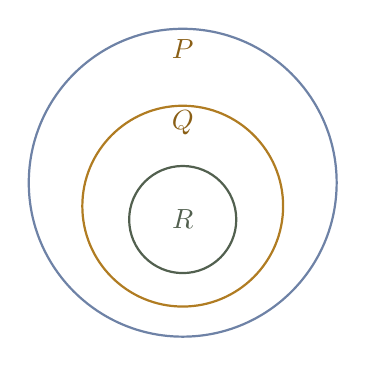
\begin{tikzpicture}[scale=0.85]
\draw[thick, indigosoft] (0,0) circle (2.3cm);
\node[goldstrong] at (0,2.0) {$P$};
\draw[thick, goldc] (0,-0.35) circle (1.5cm);
\node[goldstrong] at (0,0.9) {$Q$};
\draw[thick, inksoft] (0,-0.55) circle (0.8cm);
\node[inksoft] at (0,-0.55) {$R$};
\end{tikzpicture}
\end{center}

\small ⑴ $r\to p$ ⑵ $q\to\ \sim\!p$ ⑶ $\sim\!q\to\ \sim\!r$ ⑷ $\sim\!p\to r$\\[4pt]
\textbf{\color{goldstrong}답} \; $R\subset P$이므로 ⑴ 참. $Q\not\subset P^C$이므로 ⑵ 거짓. $Q^C\subset R^C$이므로 ⑶ 참. $P^C\not\subset R$이므로 ⑷ 거짓. \textbf{참인 명제: ⑴, ⑶}
\end{answerbox}

\section{성취수준 (이 차시 범위)}
\begin{tabularx}{\linewidth}{@{}>{\bfseries\color{goldstrong}}p{0.9cm}X@{}}
\toprule
A & 진리집합의 포함 관계로 충분조건, 필요조건, 필요충분조건을 판별하고 그 근거를 설명할 수 있다. \\
B & 진리집합의 포함 관계로 충분조건, 필요조건, 필요충분조건을 판별할 수 있다. \\
C & 충분조건, 필요조건, 필요충분조건의 뜻을 알고 간단한 경우를 판별할 수 있다. \\
D & 안내에 따라 충분조건과 필요조건을 판별할 수 있다. \\
E & 충분조건과 필요조건의 뜻을 안다. \\
\bottomrule
\end{tabularx}

\section{다음 차시}
\begin{calloutbox}
\textbf{03 명제의 증명 --- 1/2차시.} `02 명제 사이의 관계'가 여기서 마무리된다. 다음 시간부터는 대우를 이용한 증명법과 귀류법을 다룬다.
\end{calloutbox}
\end{document}
